%\begin{sidewaysfigure}
%  \begin{center}
%  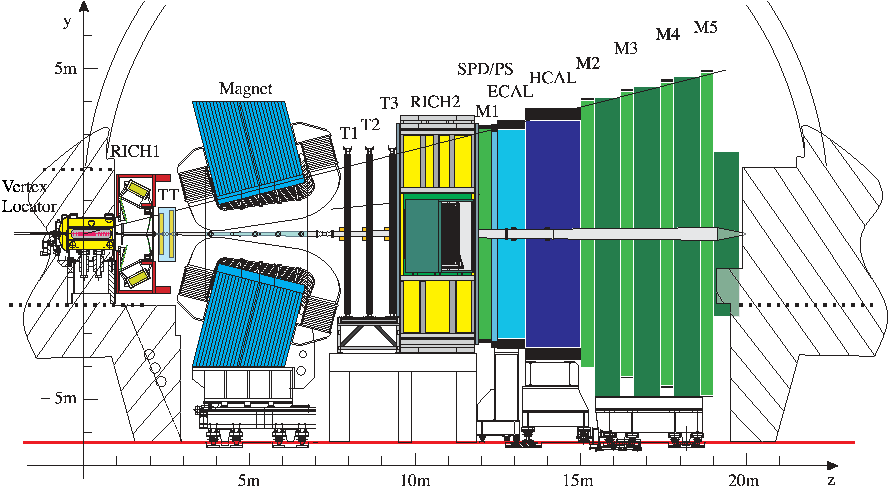
\includegraphics[width=0.8\textheight]{lhcb-detector-cross-section}
%  \caption[Cross-section view of \LHCb, cut in the non-bending $y$--$z$ plane]%
%    {Cross-section view of \LHCb, cut in the non-bending $y$--$z$ plane.}
%  \label{fig:LHCbCrossSection}
%  \end{center}
%\end{sidewaysfigure}



\chapter{ND280 software and existing ECal event reconstruction}
\label{chap:ND280Software}
The T2K experiment uses a bespoke software suite for simulation and analysis of ND280 data which is based on the ROOT framework~\cite{Brun199781}.  The vast majority of the ND280 software suite utilies these oaEvent library which provides a unified framework for information manipulation and was specifically designed for this purpose.
As ND280 consists of many subdetectors each providing a specific function, the ND280 software suite is designed to reflect this.  Not only are there specific software modules for individual subdetectors, there are specific modules for each phase of the subdetector information processing e.g. trip-T calibration, TPC reconstruction etc.  \newline
As the software suite handles both production of simulated data and the processing of collected data, there are sections of the processing chain which are specific to type of data being processed.  While the Monte Carlo simulation and real data do see different areas of the software chain, the general philosophy is to maniuplate the Monte Carlo or the real data to a point where they can be treated as equals and them process them in the same manner.  So, the description of the software will follow the same path: the Monte Carlo and real data specifics will be discussed first and then the unified treatment will follow. 
\section{Monte Carlo production software}
\label{sec:MCchain}
As described above, parts of the software chain are unique to simulated data processing.  Specifically, the simulation of the beam and the detector response need to be modelled before the Monte Carlo can be treated on equal footing with the real data.  This special processing is split into several steps, all of which are described below.

\subsection{Neutrino flux simulation}
\label{subsec:NeutrinoFluxSimulation}
The neutrino flux simulation uses Fluka2011~\cite{Ferrari_fluka:a} and a software set called JNUBEAM to model the J-PARC neutrino beam.  The process begins by using Fluka2011 to simulate the 30 GeV protons incident on the graphite target and their subsequent secondary interactions which produce the neutrino parent mesons.  The kinematic information of the hadrons is the passed to the JNUBEAM simulation.  JNUBEAM is based on GEANT3~\cite{Brun:1987ma} and models the J-PARC secondary beamline.  The hadrons are tracked through the decay volume and are allowed to interact or decay to produce the simulated neutrino beam.  Importantly, all information associated with the daughter neutrinos and their parents are saved at this point.  By storing this information, the neutrino flux can be readily re-weighted to include new information associated with beam profile measurements or external data.
\newline
The main external tuning source is NA61/SHINE which is a hadron interaction experiment that uses a 31 GeV/c proton beam colliding with changable targets~\cite{PhysRevC.84.034604}.  For use in the T2K flux simulation, NA61/SHINE has collected data using two graphite targets: one with a 4$\%$ nuclear interaction length thickness and a full T2K replica target.  The flux simulation used for this analysis is tuned using full replica target data.  Observed differences between the fluka2011 simulation and NA61/SHINE data are used to re-weight the simulated neutrino flux.
\newline
Additionally to the external data tunings measurements of the T2K beam profile are also used to re-weight the flux.  By making such measurements on a run-by-run basis, the simulated flux can be re-weighted to better model variations of the neutrino beam in each data run.
\subsection{Neutrino interaction simulation}
\label{subsec:NeutrinoInteractionSimulation}
After the neutrino flux has been modelled, simulation of the neutrino interactions with the T2K detectors follows.  The NEUT~\cite{Hayato2002171} event generator is used to simulate interactions with ND280.  The inputs to the interaction simulation are a neutrino vector file produced by the beam simulation and a ROOT based ND280 geometry.  The used geometry includes the magnetic field return yoke and everything contained within.  Using the inputs, NEUT tracks the neutrino and calculates the probability of interaction for every material in crosses.  To calculate the interation probability, the potential interaction nucleus must be modelled.  For this, NEUT uses two models; the Moniz-Smith Relativistic Fermi Gas (RFG)~\cite{Miller2002223} and the O. Benhar spectral function models~\cite{Benhar1994493}.  The spectral functions are only implemented for carbon, oxygen and iron so the model used depends on the atomic number of the interaction candidate nucleus.  It is important to note at this point that this thesis deals with neutrino interactions on lead, so it is the RFG model that is used for signal interactions.
\newline 
The main interactions modes at T2K energies are quasi-elastic scattering (CCQE), single pion production  (CC1$\pi$) and deep inelastic scattering (DIS) all of which have models in NEUT~\cite{LlewellynSmith1972261,Rein198179,1126-6708-2006-05-026}.
\newline
After the initial interactions, the final step is to simulate the final state interactions within the nucleus.  Each particle involved with the interaction is pushed through the nucleus in discreet steps with the probability of a final state interaction being calculated at each step.  If an interaction occurs, the final states of that interaction are also included in the subsequent steps.  This interative procedure models the particle cascade until all the final states have reached the nucleus boundary.  At this point, all final state particles are recorded along with all information that created those particles.  This information is stored in a vector file and passed onto the ND280 detector MC package which handles the detector's response to these final state particles.
\subsection{ND280 detector simulation}
\label{subsec:ND280DetectorSimulation}
The simulation of the final state particles in ND280 is handled by nd280mc which is based on Geant4~\cite{Agostinelli2003250} and ROOT.  The neutrino interaction vector files are taken as input and used as seeds in the detector simulation.  The neutrino vector inputs are not organised according to the J-PARC beam bunch structure so the detector simulation first groups the interactions into spills.  The beam intensity being simulated is used to define how many interactions occur in a spill with Poisson fluctuations applied to that number.  The timing of the beam bunch structure is then used to group the interactions into bunches. 
\newline
nd280mc constructs a ROOT geometry of ND280 based on the design specifications of its subdetectors and then propagates the particles given to it by the neutrino generator through the geometry, simulating energy deposition, scattering and particle decay during propagation.

\subsection{Detector response simulation}
\label{subsec:DetectorResponseSimulation}
Is elecSim there?

\subsection{Detector calibration}
\label{subsec:DetectorCalibration}
oaCalib calibrates

\subsection{Event reconstruction}
\label{subsec:EventReconstruction}
oaRecon yo!


\section{Real data processing software}
\label{sec:datachain}
Process the data.  MAY NOT INCLUDE THIS


\section{ECal event reconstruction}
\label{sec:ECalEventReconstruction}
All about ecalRecon

\subsection{Hit preparation}
\label{subsec:ECalHitPerparation}
Hit prep

\subsection{Basic clustering}
\label{subsec:ECalBasicClustering}
Baaasic

\subsection{Cluster combination}
\label{subsec:ECalCombineClusters}
Combine dem clusters

\subsection{Cluster expansion}
\label{subsec:ECalExpandClusters}
Expand dem clusters

\subsection{3D cluster formation}
\label{subsec:ECal3DMatching}
Match the clusters

\subsection{3D hit reconstruction}
\label{subsec:ECal3DHitReconstruction}
Least square those fits

\subsection{Energy reconstruction}
\label{subsec:ECalEnergyReconstruction}
blah

\subsection{Event classification}
\label{subsec:ECalParticleIdentification}
Track or shower?
